\section{E-MOS Analytical Model}\label{sec:analytic}

\begin{figure}[h]
  \begin{center}
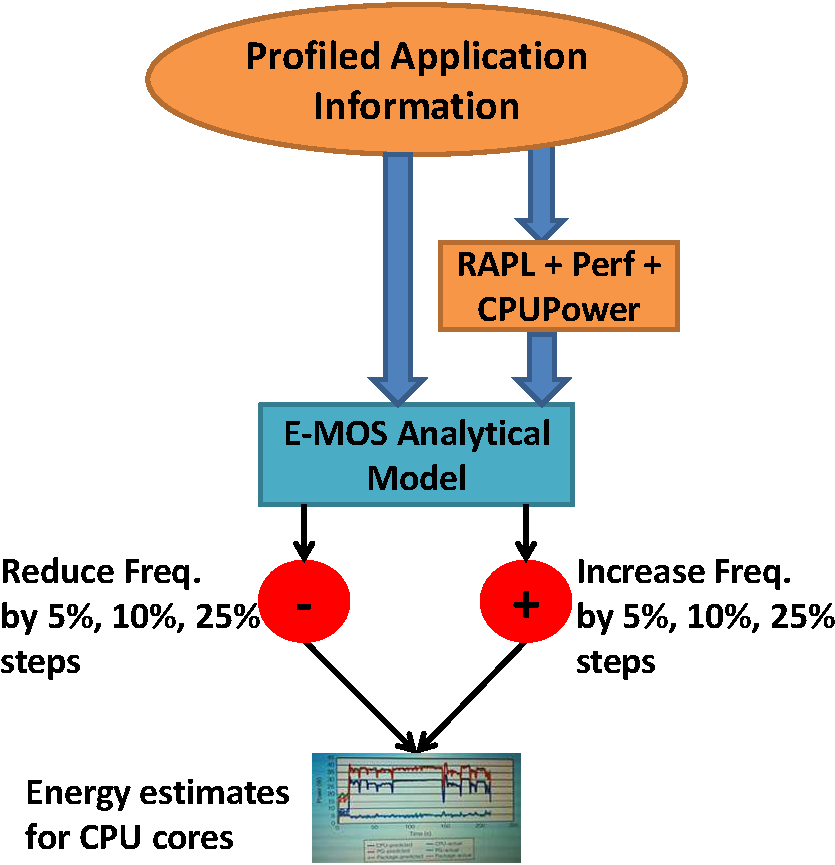
\includegraphics[width=\linewidth]{figs/EMOS-new-crop.pdf}
  \end{center}
  \vspace{-0.1in}
  \caption{a) E-MOS model; b) Frequency setting in User-space governor}
	\label{fig:emos-model}
\end{figure}


With the detailed analysis and reasoning out the anomalies 
of existing power governors in the previous section, we now present our 
E-MOS (Efficient Energy Management Policies in OS) analytic model
which mainly relies on the principle of application-aware energy management. 
We believe that OS providing more freedom to user-space for energy
management is beneficial, since user-space has more relevant information about applications
and their behavior. Ofcourse, dynamic power management by changing the CPU frequency and 
DRAM frequency simultaneously based on application phases would be an ideal 
power governor behavior. But, our model as of now only statically decides a frequency setting 
based on overall application characteristic. Although, E-MOS is an analytical model,
one could modify the existing OS power governor to implement E-MOS. Our project
aims to evaluate E-MOS model with variety of applications, and based on the results
and analysis we aim to modify the power governor and do dynamic power management.

Figure~\ref{fig:emos-model} \textcolor{red}{(a)} depicts the overview
of our E-MOS model. It takes the profiled application information -- number of 
compute, cache sensitive, memory intensive instructions (Profiling output from PIN model) as input 
and uses Linux utilities to get the execution time (\texttt{perf}), energy (\texttt{perf} and \texttt{RAPL}) and 
frequency (\texttt{CPUPOWER}) estimates with the
default power governors. These application level measurements are then used 
by a python framework model and it gets the new energy estimates
by increasing or reducing the frequency by 10\%, 15\% and 25\% scaling steps.
The model, estimates the energy based on the runtime statistics collected for the application and equation below:
\newline
\newline
\begin{math}
\centering
{Energy (E) = Power (P) * Execution Time (T)}
\end{math}
\newline

\begin{figure}[h]
  \begin{center}
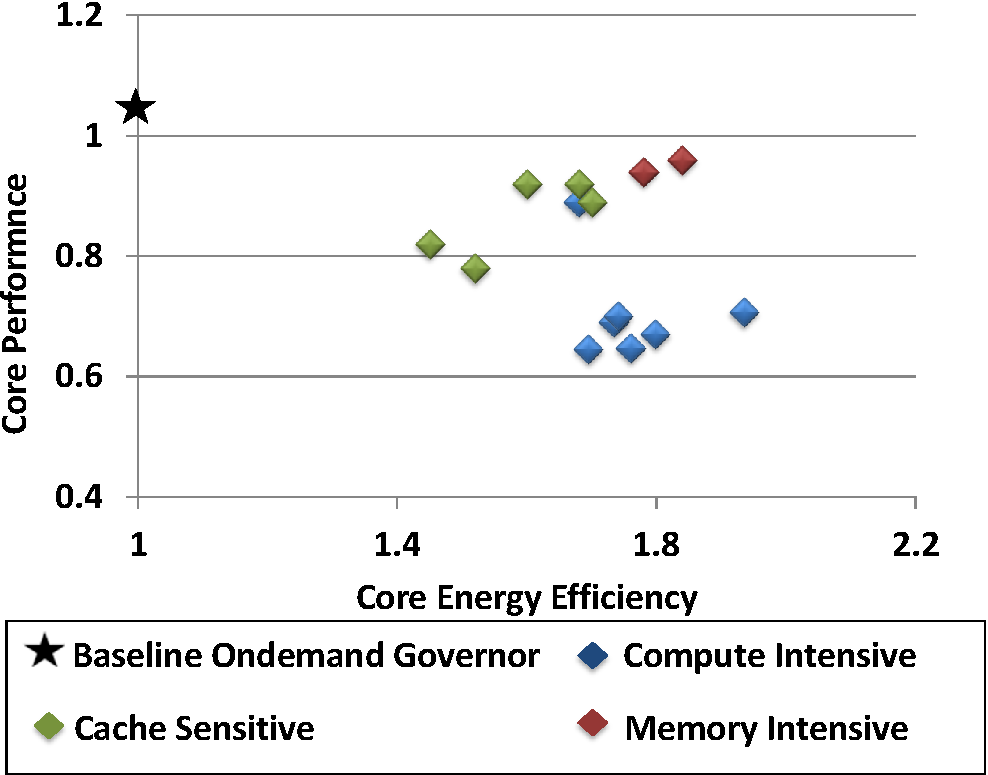
\includegraphics[width=\linewidth]{figs/ana-reduce-crop.pdf}
  \end{center}
  \vspace{-0.1in}
  \caption{Energy estimates from E-MOS when frequency reduced by 30\% (600Mhz)}
	\label{fig:reduce-freq}
\end{figure}

Power is measured by \texttt{RAPL} utility again with the varied frequency 
and execution time with \texttt{perf}. These new energy estimates are then plotted
with ondemand power governor as baseline. 
Figure~\ref{fig:reduce-freq} and Figure~\ref{fig:increase-freq}
shows one such example of E-MOS reducing and increasing the CPU core frequency by 25\% (600 Mhz).
Ideally, you want to vary both CPU core and DRAM frequency for different application types
and then evaluate over baseline model. But, current Linux APIs are not sophisticated
enough to measure the runtime frequency and energy estimates for DRAM. Also, there is very limited
interface to modify the runnable frequency of DRAM.


\begin{figure}[h]
  \begin{center}
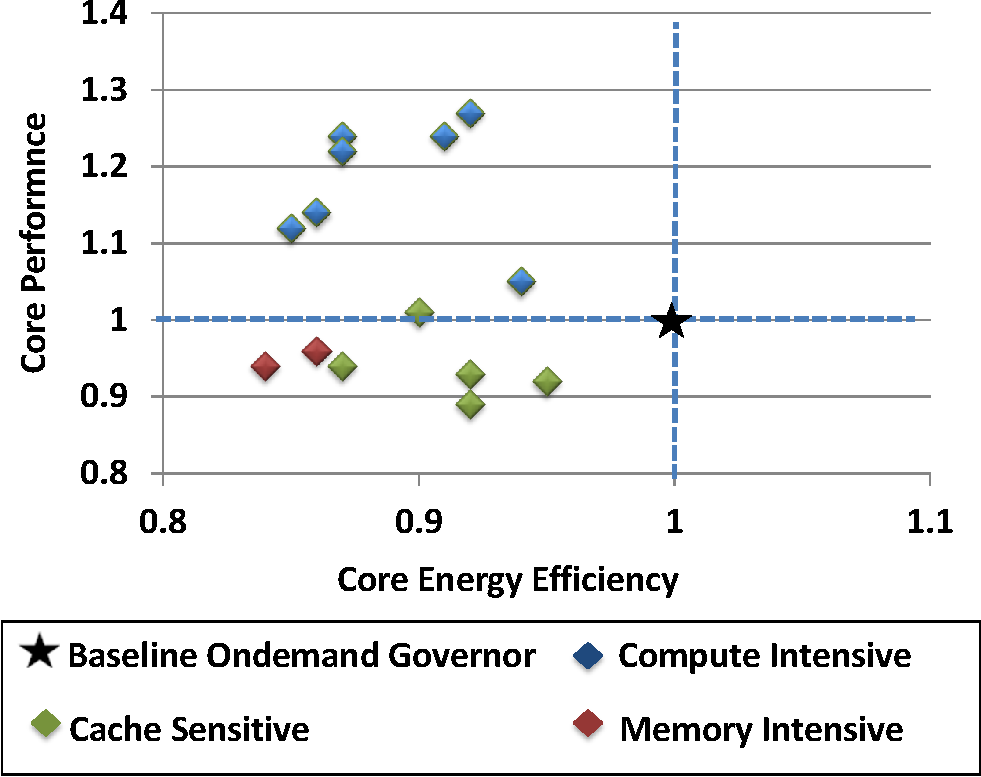
\includegraphics[width=\linewidth]{figs/ana-increase-crop.pdf}
  \end{center}
  \vspace{-0.1in}
  \caption{Energy estimates from E-MOS when frequency increased by 30\% (600Mhz)}
	\label{fig:increase-freq}
\end{figure}

\subsection{Core frequency reduction}
Figure~\ref{fig:reduce-freq}, plots all the applications
with their performance on y-axis and core energy efficiency on x-axis
normalized to ondemand governor. We can see that the energy efficiency
of all the applications increases significantly upto 1.9x with the core frequency reduction by 600Mhz.
But, the performance of compute intensive applications takes a hit, as they mainly depend on   
core frequency. Interestingly, memory intensive applications performance is very close to ondemand
governor as they do not much depend on core frequency. Even, cache sensitive applications
lose only around 15\% performance with such a large core frequency reduction. This, indicates that
there is potential in energy efficiency gain while executing  cache sensitive and memory intensive applications 
by reducing the core frequency. 

\subsection{Core frequency increase}
Figure~\ref{fig:increase-freq}, shows a scenario
where the core frequency is increased by 600Mhz.
Here, compute intensive application have speedup upto 1.25x which
is expected. But, there is no much speedup improvement for cache and memory applications
with the increase in core frequency. This, indicates that, increasing core frequency
has no much effect on performance of memory and cache applications and you might not want to decrease
core frequency when executing memory and cache applications to gain better energy efficiency.

\subsection{E-MOS energy management policies}
Now, based on the E-MOS model energy results for various applications, and different frequency 
settings, we formulated a policy decision table to be followed by the power governors based on the 
application type and the objective. These policies are formulated based on
the energy estimates from the E-MOS model. Table~\ref{tbl:emos-dec} shows the policy
decisions to be taken for various applications based on the energy or performance objective.
Even though, E-MOS model does not control or evaluate DRAM frequency, based on the energy estimated
for two scenarios mentioned above, we formulated the policies for DRAM frequency setting too.
All our further evaluations and results only uses core frequency setting policies and all the evaluation is
optimized for energy as the first class constraint. Figure~\ref{fig:emos-model} \textcolor{red}{(b)} shows
how based on the suggested frequency setting of E-MOS model, user-application can scale the CPU core
frequency setting using user-space power governor. With user-space power governor one can manually set the core frequency
and pin the application to run with that. Thus, E-MOS model along with the user-space power governor
can act as n application-aware energy management tool, for better energy efficiency. 

\begin{table}[h]
\footnotesize
\def\arraystretch{0.52}
\setlength{\tabcolsep}{.15em}
\center
\begin{tabular}{cccc} \toprule
Application & Objective & CPU Freq. & DRAM Freq.  \\ \midrule
Compute & Energy & Maintain\textbackslash{Increase} & Decrease \\
Compute & Performance & Increase & Maintain \\
Cache  & Energy &  Decrease & Decrease \\ 
Cache  & Performance &  Maintain & Increase \\ 
Memory & Energy & Decrease & Maintain\textbackslash{Increase} \\
Memory & Performance & Maintain & Increase \\ \midrule
\end{tabular}
\caption{E-MOS Policies Decision Table}\label{tbl:emos-dec}
\end{table}

\subsection{Limitations}
We believe our first order E-MOS model, is preliminary model
and lot of improvements are needed to more dynamic power management. 
Once such scenario is where a single application has multiple execution phases with compute and memory intensive
and you need support to dynamically switch to the corresponding phase by increasing/decreasing the core and DRAM
frequency. Also, since this is an analytical model, more realistic estimates can be obtained 
by integrating this model inside an actual kernel power governor. We aim to implement this as future work.
